\chapter{Transformation de Fourier discrète}
Une telle TF va nous permettre d'estimer une TF continue en différents points. C'est par 
exemple ce que fait un ordinateur pour afficher les pixels. 
\section{Définition}
Considérons un signal périodique $x(n)$ de période $N$
\begin{equation}
x(n) = x(n+lN)\qquad l =0,1,2,3,\dots
\end{equation}
Celui-ci possède une TF discrète
\begin{equation}
x(n) = \frac{1}{N}\sum_{k=0}^{N-1} X(k)e^{j\frac{2\pi}{N}kn}\quad\rightarrow\text{TF discrète inverse}
\end{equation}
La relation inverse permet le calculer les valeurs $X(k)$
\begin{equation}
X(k) = \sum_{n=0}^{N-1} x(n)e^{-j\frac{2\pi}{N}nk} \rightarrow\text{TF discrète}
\end{equation}
Ce $X(k)$ est aussi périodique, de période $N$
\begin{equation}
\begin{array}{lll}
X(N) &= X(0) = X(lN)\\
X(N+1) &= X(1) = X(lN+1)\\
X(k) &= X(k+lN)
\end{array}
\end{equation}
L’Intérêt de la TF discrète est l'utilisation d'algorithme comme \texttt{FFT}. Notons que 
$x(n), X(k)$ et $e^{j\frac{2\pi}{N}nk}$ étant périodiques, on peut remplacer les sommes de 
0 à $N-1$ par des sommes de $n_l$ à $n_l+N-1$.

\section{Propriétés de la DFT}
Je ne reprends ici que les plus intéressantes ou celles qui peuvent être commentées. Cependant 
attention, ce sont souvent des questions d'examen.

	\subsection{Linéarité et glissement}
	Voir slide T3. Pour le glissement, on ne doit pas prendre de 0 à $N-1$ mais simplement 
	"une suite". 
	
	\subsection{Convolution périodique}
	Voir slide T4
	
	\subsection{Propriétés de symétrie}
	Pour les deux premières propriétés, voir slide T5. Pour la troisième ;\\
	\textit{On peut obtenir les DFT de deux séquences réelles en calculant la DFT d'une séquence 
	complexes.} Si $x_1(n)$ et $x_2(n)$ sont réelles, on peut obtenir
	\begin{equation}
	\left\{\begin{array}{ll}
	x_1(n) &\ft X_1(k)\\
	x_2(n) &\ft X_2(k)	
	\end{array}\right.\quad\Rightarrow\quad x_1(n)+jx_2(n) \ft X(k)
	\end{equation}
	Nous avons donc fabriqué un signal avec une partie réelle et une partie imaginaire. Une seule 
	transformée de Fourier permet d'obtenir les deux signaux
	\begin{equation}
	X_1(k) = \frac{1}{2}[X(k)+X^*(N-k)],\qquad 	X_2(k) = \frac{1}{2j}[X(k)-X^*(N-k)]	
	\end{equation}
	
	\begin{proof}\ \\
	Par linéarité
	\begin{equation}
	x_1(n)+jx_2(n) \ft X_1(k)+jX_2(k) = X(k)
	\end{equation}
	Par la première propriété de symétrie ($x(n)\ft X(k)$ et $x^*(n)\ft X^*(-k)$)
	\begin{equation}
	x^*(n) = x_1(n) -jx_2(n) \ft X_1(k)-jX_2(k) = X^*(-k)=X^*(N-k)
	\end{equation}
	\end{proof}
	
	\subsection{Formule de Pascal}
	Ceci est typiquement une question d'examen. La formule de Pascal nous dit que l'énergie dans 
	le domaine temporel est la même que dans le domaine fréquentiel. 
	\begin{equation}
	\sum_{n=0}^{N-1} |x(n)|^2 = \frac{1}{N}\sum_{k=0}^{N-1} |X(k)|^2
	\end{equation}
	\begin{proof}\ \\
	L'astuce consiste à exprimer $x^*(n)$ à l'aide de la TF inverse
	\begin{equation}
	\begin{array}{ll}
	\DS\sum_{n=0}^{N-1} |x(n)|^2 &= \DS\sum_{n=0}^{N-1}x(n)x^*(n) = \sum_{n=0}^{N-1}x(n)\left[
	\frac{1}{N}	\sum_{k=0}^{N-1}X(k)e^{j\frac{2\pi}{N}kn}\right]^*\\
	&=\DS \sum_{n=0}^{N-1}x(n)\frac{1}{N}\sum_{k=0}^{N-1}X^*(k)e^{-j\frac{2\pi}{N}kn}\\
	&=\DS \frac{1}{N}\sum_{k=0}^{N-1}X^*(k)\sum_{n=0}^{N-1}x(n)e^{-j\frac{2\pi}{N}kn}\\
	&=\DS\frac{1}{N}\sum_{k=0}^{N-1}X^*(k)X(k) = \frac{1}{N}\sum_{k=0}^{N-1} |X(k)|^2
	\end{array}
	\end{equation}
	\end{proof}
	
	\exemple{ Nous avons un signal numérique au spectre continue. Le but est d'exprimer ce 
	spectre en un nombre de points définis. Calculons donc la DFT du signal périodique $f(n)$, 
	de période $N$, dont une période est définie par
	\begin{equation}
	f(n) = e^{j\omega_0n}\qquad 0\leq n\leq N-1
	\end{equation}
	Ce choix nous permet de tester un large range de fréquence en faisant varier $\omega_0$. On 
	obtient alors
	\begin{equation}
	F(k) = \sum_{n=0}^{N-1}e^{j\omega_0n}e^{-j\frac{2\pi}{N}nk} = \sum_{n=0}^{N-1}\alpha^n = 
	\dfrac{1-\alpha^N}{1-\alpha}\qquad \alpha\neq1
	\end{equation}
	Imposons deux valeurs pour $\omega_0$.
	\begin{enumerate}
	\item
	$$\omega_0 = q\dfrac{2\pi}{N}\quad\Leftrightarrow\quad q = \dfrac{\omega_0N}{2\pi}$$
	où $q$ est entier. Notre signal est juste périodique de période $N$. On obtient alors
	$$\alpha = e^{j\frac{2\pi}{N}(q-k)}\quad \text{et}\quad \alpha^N = 1\qquad \forall k$$
	On obtient par contre $\alpha=1$ si $q=k$. Dès lors
	\begin{equation}
	\begin{array}{lll}
	F(k) &= N&\quad \text{si } k=q\\
	&= 0\quad \text{si } k\neq q\\
	\end{array}
	\end{equation}
		\begin{center}
		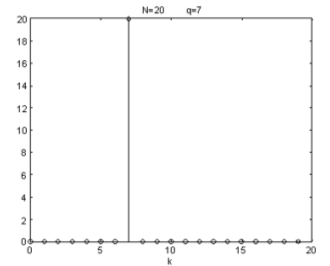
\includegraphics[scale=0.4]{ch5/image1}
	\captionof{figure}{Le spectre ne fait ressortir qu'une seule fréquence : le signal n'en 
	contient donc qu'une seule.}
	\end{center}
	On s'en doute, obtenir une seule fréquence est un cas particulier. Dans la majorité des 
	cas ce n'est pas le cas. C'est ce que nous allons maintenant voir

	\end{enumerate}}
	\newpage
	\exemple{
	\begin{itemize}
	\item[2]
		\item
	$$\omega_0 = x\dfrac{2\pi}{N}\qquad\rightarrow\qquad\alpha = e^{j\frac{2\pi}{N}(x-k)}$$
	où $x$ n'est \textbf{pas} entier. En appliquant la suite géométrique
	\begin{equation}
	F(k) =\DS \frac{1-\alpha^N}{1-\alpha} = \dots = e^{j\frac{\pi}{N}(N-1)(x-k)}\dfrac{\sin(
	\pi(x-k))}{\sin(\pi(x-k)/N)}
	\end{equation}
	Ici, tous les échantillons de $F(k) \neq 0$.
			\begin{center}
		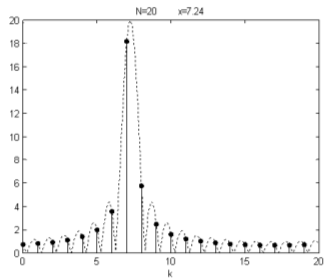
\includegraphics[scale=0.4]{ch5/image2}
	\captionof{figure}{Le spectre ressemble à un sinus cardinal mais échantillonné à certains 
	points. On voit quand même une certaine périodicité se dégager mais avec une assez grande 
	incertitude.}
	\end{center}
	\end{itemize}}
	
\section{Applications de la DFT}
	\subsection{Évaluation de la TF d'une séquence finie}
		\begin{wrapfigure}[8]{l}{5.5cm}
	\vspace{-5mm}
	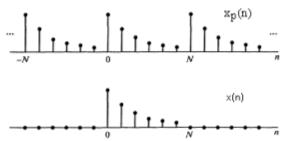
\includegraphics[scale=0.5]{ch5/image3.png}
	\captionof{figure}{On peut copier coller l'un sur l'autre.}
	\end{wrapfigure}	
	Soit une séquence \textbf{finie} d'une seule période du signal périodique $x_p(n)$ et 
	nul ailleurs :
	\begin{equation}
	\begin{array}{lll}
	x(n) &= x_p(n)&\quad 0\leq n\leq N-1\\
	&=0&\quad\text{sinon}
	\end{array}
	\end{equation}
	La TF ($\neq$ DFT) de la séquence finie $x(n)$ donne un spectre continu
	\begin{equation}
	X(e^{j\omega}) = \sum_{n=-\infty}^\infty x(n)e^{-j\omega n} = \sum_{n=0}^{N-1} x_p(n)
	e^{-j\omega n}
	\end{equation}
	Considérons maintenant la DFT de $x_p(n)$, $X_P(k)$ :
	\begin{equation}
	X_p(k) = X(e^{j\omega})|_{\omega=k\frac{2\pi}{N}}
	\end{equation}
	On retombe sur la même chose, c'est la définition de la DFT. La DFT d'un séquence périodique 
	fournit donc une évaluation de la transformée de Fourier de la séquence finie associée, en $N$ 
	points régulièrement répartis sur l'axe des fréquences, entre $\omega=0$ et $\omega=2\pi$. En 
	conclusion, cela revient à évaluer le spectre continu à intervalle régulier grâce à la DFT.\\
	
	Pour une séquence finie de longueur $N$, DFT permet d'évaluer la TF en un nombre de  points 
	\textbf{plus grand que $N$} : on va échantillonner en fréquence, mais prendre un échantillon 
	plus petit. Soit une tel séquence finie
	\begin{equation}
	x(n) \quad \text{for} \quad 0\leq n \leq N-1
	\end{equation}
	Sa TF est 
	\begin{equation}
	X(e^{j\omega}) = \sum_{n=0}^{N-1} x(n)e^{-j\omega n}
	\end{equation}
	La DFT permet de calculer $X(e^{j\omega})$ de façon efficace : on calcule en certains points 
	et on particularise à $\omega=\frac{2\pi}{L}l$. Exprimons $X(e^{j\omega})$ en $L$ point uniformément 
	répartis entre 0 et $2\pi$.
	\begin{equation}
	X\left(e^{j\frac{2\pi}{L}l}\right) = \sum_{n=0}^{N-1}x(n)e^{-j\frac{2\pi}{L}ln}\qquad l=0,\dots,L-1
	\end{equation}
	Définissions $\tilde{x}(n)$ qui prolonge $x(n)$ avec des zéros
	\begin{equation}
	\begin{array}{lll}
	\tilde{x}(n) &= x(n) &\quad 0\leq n\leq N-1\\
	&=0&\quad N\leq n\leq L-1
	\end{array}
	\end{equation}
	Calculons la DFT de ce signal (ou plus exactement la DFT du signal périodique, de période $L$,
	dont $x(n)$ représente une période). Celle-ci est facile à calculer, le signal étant nul entre 
	$N-1$ et $L-1$
	\begin{equation}
	\begin{array}{ll}
	\tilde{X}_p(k) &=\DS \sum_{n=0}^{L-1} \tilde{x_p}(n)e^{-j\frac{2\pi}{L}nk} = \sum_{n=0}^{N-1} 
	x(n)e^{-j\frac{2\pi}{L}nk}\\
	&=\DS X\left(e^{j\frac{2\pi}{L}k}\right)
	\end{array}
	\end{equation}
	La DFT est de nouveau l'estimation de $x(n)$ en $L$ points. Ceci constitue une technique simple pour 
	calculer la transformée de Fourier d'une séquence finie en un grand nombre de points (choisis).
	
	
	\subsection{Inversion d'une transformée de Fourier}
		\subsubsection{Séquence finie}
		Soit les échantillon $x(n)$ d'une séquence finie dont les $N$ valeurs sont prises à intervalles 
		réguliers entre $\omega=0$ et $\omega=2\pi$. On a vu que si on donne $N$ valeurs de $X_p(k)$, 
		on peut trouver $x(n)$ tel que sa TF prenne les valeurs de $X_p(k)$ imposées aux $N$ points\footnote{
		Uniformément réparti sur l'axe des fréquences.} (problème d'interpolation). La TF est (ici la somme 
		est bien finie, on prend $N$ points de la séquence finie et continue)
		\begin{equation}
		X(e^{j\omega}) = \sum_{n=0}^{N-1} x(n)e^{-j\omega n}
		\end{equation}
		Les $N$ valeurs sur le cercle unité sont 
		\begin{equation}
		X(e^{j\frac{2\pi}{N}k}) = X_p(k)\qquad k=0,\dots,N-1
		\end{equation}
		On exprime la séquence $x(n)$ par
		\begin{equation}
		x(n) = \frac{1}{N}\sum_{n=0}^{N-1} X_p(k)e^{j\frac{2\pi}{N}kn}\qquad n=0,\dots,N-1
		\end{equation}
		La TF d'une séquence finie est entièrement déterminée par ses $N$ valeurs régulièrement 
		réparties sur l'axe des fréquences.
	
	
		\subsubsection{Séquence infinie}
		On s'intéresse maintenant à la transformation de Fourier continue évaluée en $N$ points : 
		nous allons voir à quoi cela correspond en temporel. On obtiendra un "copié-collé" fini du 
		signal infini.\\
		Considérons une séquence $h(n)$ pouvant être infinie ainsi que sa TF
		\begin{equation}
		H(e^{j\omega}) = \sum_{n=-\infty}^\infty h(n)e^{-j\omega n}
		\end{equation}
		L'information est exprimée en une infinité de points : n'en prendre que $N$ serait louper 
		quelque chose. Néanmoins, évaluons $H(e^{j\omega})$ en $N$ (ici arbitraires, le signal est 
		infini), mais uniformément répartis sur l'axe des fréquences
		\begin{equation}
		H_p(k) = H(e^{j\omega})|_{\omega=k\frac{2\pi}{N}} = \sum_{n=-\infty}^\infty h(n)e^{-j\frac{2\pi}{
		N}kn}
		\end{equation}
\vspace{-5mm}
			\begin{wrapfigure}[22]{l}{7cm}
		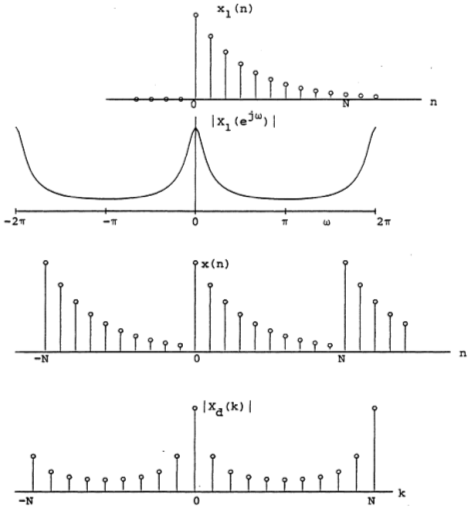
\includegraphics[scale=0.4]{ch5/image4}
		\captionof{figure}{Le premier graphique est notre signal qui tend vers zéro (pour des raison 
		de convergence) sans jamais l'atteindre. Le second est le spectre, comme d'habitude. Le troisième 
		est construit comme une répétition de $x_1(n)$ que l'on a copié-collé. On remarque que 
		$x(n-1)$ est un peu plus grand ici : ceci vient de toutes les petites contributions tendant vers 
		zéro que l'on a sommé. Le dernier est un spectre à raie où l'on a pris $k$ échantillons 
		uniformément réparti sur l'axe des fréquences.}
	\end{wrapfigure}	
		La dernier membre est la série de Fourier d'un signal $h_p(n)$ périodique construit à partir d'un 
		signal non périodique $h(n)$ : c'est ce que nous avions vu au chapitre 3 ! On va alors procéder 
		à un copié-collé infini pour trouver un signal périodique d'ordre $n$
		\begin{equation}
		h_p(n) = \frac{1}{N}\sum_{k=0}^{N-1} H_p(k)e^{j\frac{2\pi}{N}nk} = \sum_{r=-\infty}^\infty h(n+rN)
		\end{equation}
		D'autre part
		\begin{equation}
		x(n) = \sum_{r=-\infty}^\infty x_1(n+rN) \ft X_d(k) = X_1(e^{j\frac{2\pi}{N}k})
		\end{equation}
		On ne retombe pas sur le signal initial mais sur un autre : le copié-collé du signal initial 
		de façon infinie. Si par hasard les coefficients valent zéro en dehors de l'intervalle 
		ci-dessous, on n'a plus d'overlap.
		\begin{equation}
		h_p (n) = h(n)\qquad 0\leq n \leq N-1
		\end{equation}
		On retrouve le cas précédent. Si ce n'est pas le cas, on aura recouvrement entre les différents 
		$h(n)$ décalés : on peut le réduire en augmentant $N$.

		
	
	
	\newpage
	\section{Analyse de Fourier par DFT}
	On cherche à réaliser le système suivant en labo.
	\begin{center}
	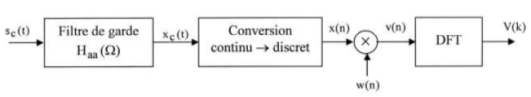
\includegraphics[scale=0.54]{ch5/image5}
	\captionof{figure}{\ }
	\end{center}
	Le filtre de garde est la pour éviter le repliement spectrale. Ensuite, il faut convertir le signal 
	continu en signal discret $(x_c(nT)=)x(n)$. Pour obtenir le spectre, on multiplie ce signal continu par une 
	fonction, par exemple fenêtre, $w(n)$.  Le spectre continu vaut
	\begin{equation}
	X(e^{j\omega}) = \frac{1}{T}\sum_{r=-\infty}^\infty X_c\left(\frac{\omega}{T}+r\frac{2\pi}{T}\right)
	\end{equation}
	On espère que le filtre de garde va couper de $-\pi$ à $\pi$ pour n'obtenir que le spectre qui 
	nous intéresse de façon à ce qu'il ne soit pas spoilé par les spectres décalés
	\begin{equation}
	X(e^{j\omega})\approx \frac{1}{T}X_c\left(\frac{\omega}{T}\right)\qquad -\pi<\omega<\pi
	\end{equation}
	On cherche à évaluer $X_c(\Omega)$ avec la DFT (évaluation en $N$ points). Ce n'est pas exactement 
	le signal $S_C(\Omega)$ à cause du filtre de garde (car coupe les fréquences, mais on considère que 
	ces fréquences coupées sont sans intérêts).\\
	
	Évaluer $X_c(\Omega)$ revient à évaluer $X(e^{j\omega})$ qui est la TF d'un signal à TD de durée
	non limitée
	\begin{equation}
	X(e^{j\omega}) = \sum_{n=-\infty}^\infty x(n)e^{-j\omega n}
	\end{equation}
	
	\begin{wrapfigure}[17]{r}{5.7cm}
	\vspace{-5mm}
	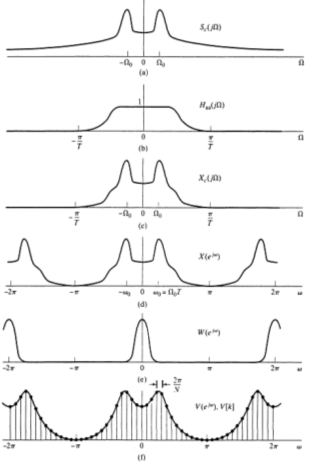
\includegraphics[scale=0.45]{ch5/image6}
	\captionof{figure}{\ }
	\end{wrapfigure}	
	Pour la DFT, il faut que la séquence temporelle soit limitée : on prend $N$ échantillon où $N$ 
	peut être grand, mais pas infini. Le signal $w(n)$ que l'on multiplie à $x(n)$ permet 
	d'obtenir une séquence de durée finie
	\begin{equation}
	\begin{array}{ll}
	v(n) &= w(n).x(n)\\
	w(n) &=0\qquad n<0\text{ et } n\geq N
	\end{array}
	\end{equation}
	
	Ceci à le même effet qu'une fonction fenêtre qui sert bien à "couper dans le temps".\\
		
	Le signal $(a)$ est le signal de départ. Comme tout signal, son spectre s'étend jusqu'à l'infini. 
	Problème : si on ne peut pas négliger le repliement spectral, il est nécessaire d'utiliser un 
	filtre de garde $(b)$ (qui a ici une allure réelle). L'application de ce filtre de garde donne 
	$(c)$. On voit que les hautes fréquences ont été atténuées. Il faut ensuite passer dans le domaine 
	numérique $(d)$ : le spectre a été copié-collé indéfiniment. Heureusement, dans le continu, le 
	spectre s'arrêtait à $\pi/T$, il s'arrête donc à $\pi$ dans le numérique.\\

\newpage
	 On multiplie (\!!)\footnote{
	Si on avait fait la convolution ça aurait été le produit des deux. Ici on fait un PRODUIT au niveau 
	temporel donc en spectre on a une convolution.} notre signal $x(n)$ par un autre signal qui lui est
	rectangulaire (fenêtre). Le $(e)$ est le spectre de la fonction fenêtre. Nous allons gentillement 
	"lisser" le spectre initial par la fonction fenêtre, on peut en effet voir que celui-ci $(f)$ est 
	plus lisse. Pourquoi une fonction fenêtre ? On voit un désavantage car on n'a plus le spectre de départ, 
	on veut donc minimiser l'effet. En pratique on est obligé de réaliser numériquement, estimer 
	numériquement la TF en un nombre de points fini. Comme on ne peut pas mettre de signal de durée infinie, 
	il était nécessaire de "couper le temps" avec une telle fonction.\\
	
	La fonction fenêtre la plus comme toi, simple, est la rectangulaire
	\begin{equation}
	\begin{array}{lll}
	w(n) &= 1&\qquad n=0,\dots,N-1\\
	&=0&\qquad\text{sinon}
	\end{array}
	\end{equation}
	La DFT de longueur $N$ de $v(n)$
	\begin{equation}
	V(k) = \sum_{n=0}^{N-1} v(n)e^{-j\frac{2\pi}{N}nk}\qquad k=0,\dots,N-1
	\end{equation}
	Or, $v(n)$ est de longueur finie ($N$)
	\begin{equation}
	V(k) = V(e^{j\omega})|_{\omega=k\frac{2\pi}{N}}
	\end{equation}
	Même chanson : on évalue le spectre en $N$ points et on a toute l'information nécessaire. Dis 
	plus formellement : la DFT $V(k)$ correspond donc à l’échantillonnage de $V(e^{j\omega})$ en $N$ points
	uniformément répartis. Chaque échantillon correspond à une fréquence réduite et est donc à temps 
	continu\footnote{Pq?}.\\
	
	Notre but d'évaluer $X$ nous permet d'évaluer $V$ (après fenêtre). Comme $v(n)=x(n).w(n)$, il suffit 
	de faire la convolution périodique des spectres
	\begin{equation}
	V(e^{j\omega}) = \dfrac{1}{2\pi}\int_{-\pi}^\pi X(e^{j\theta}).W(e^{j(\omega-\theta)})\ d\theta
	\end{equation}
	$V$ sera alors une version "lissée" de $X$. Nous allons examiner deux effets différents dus à 
	l'utilisation de la DFT pour évaluer $X_c$
	\begin{enumerate}
	\item L'effet de la fenêtre temporelle (passage de $X$ à $V$)
	\item L'effet de l’échantillonnage fréquentiel (Passage de $V(e^{j\omega})$ à $V(k)$).
	\end{enumerate}
		
		\subsection{Effet de la fenêtre}
		Supposons que $s_c(t)$ soit la somme de deux cosinus
		\begin{equation}
		s_c(t) = A_0\cos(\Omega_0t+\theta_0)+A_1\cos(\Omega_1t+\theta_1)
		\end{equation}
		On suppose que l'on se trouve dans la bande passante du filtre de garde
		\begin{equation}
		x(n) = A_0\cos(\Omega_0n+\theta_0)+A_1\cos(\Omega_1n+\theta_1)
		\end{equation}		
		où $\omega_0=\Omega_0T$ et $\omega_1 = \Omega_1T$. On \textbf{multiplie} par la fonction 
		fenêtre
		\begin{equation}
		v(n) = A_0w(n)\cos(\Omega_0n+\theta_0)+A_1w(n)\cos(\Omega_1n+\theta_1)
		\end{equation}
		En écrivant les cosinus avec des exponentielles complexes et en appliquant le décalage 
		dans le temps, on trouve
		\begin{equation}
		V(e^{j\omega}) = \frac{A_0}{2}e^{j\theta_0}W(e^{j(\omega-\omega_0)})+
		\frac{A_0}{2}e^{-j\theta_0}W(e^{j(\omega-\omega_0)})+
		\frac{A_0}{2}e^{j\theta_1}W(e^{j(\omega-\omega_1)})+
		\frac{A_0}{2}e^{-j\theta_1}W(e^{j(\omega-\omega_1)})
		\end{equation}
		On voit que ces quatre composantes \textbf{dépendent} de la fonction fenêtre.\\
		
		\exemple{Les slides T7 à T10 reprennent un bel exemple, que je me contente de commenter ici. 
		\begin{description}
		\item[T7] Il s'agit de la fonction sinc. Aux extrémités, le bruit est $\pm$ constant.
		\item[T8]  On observe quatre pics de résonance sur le premier graphiques, bien distincts. Mais, 
		la fenêtre ayant une influance sur le spectre, si celle-ci est mal choisie les pics vont se 
		rapprocher et leurs amplitudes vont s'influencer l'une l'autre : c'est le phénomène de 
		dispersion.
		\item[T9] Les deux pics sont devenu trop proche, il n'y a plus qu'un seul maximum : la résolution 
		est devenue trop faible, il n'y a plus qu'une seule fréquence distinguable alors qu'il y en 
		avait deux au départ. Mauvaise fenêtre donc!
		\end{description}
		Le dernier slide (T10) ne demande pas de commentaires particuliers.}\ \\
		
		Les slides T11 à T16 illustrent les différentes fonctions fenêtres. Une lecture attentive suffira.
		
		
		\subsection{Effet de l'échantillonnage fréquentiel}
		On sait que la DFT échantillonne $V(e^{j\omega})$ (continu) aux fréquences $\omega_k = k
		\frac{2\pi}{N}$ où $k=0,\dots,N-1$. Le souci est que parfois $\omega_k$ ne tombe pas exactement 
		sur les extréma de $V(e^{j\omega})$ et estimer les amplitudes du signal d'entrée à partir 
		des amplitudes de la DFT est parfois compliqué. \\
		
		Il n'y a que pour un cas \textbf{particulier} où les fréquences d'entrées sont un multiple de 
		$2\pi/N$ que la DFT sait identifier les fréquences exactement.
		
			\subsubsection{Illustration du cas particulier}
			Considérons la même somme de cosinus que précédemment avec $A_0=1,A_1=0.75, \theta_0=\theta_1
			=0$. Prenons $N=64$ comme longueur de la fenêtre rectangulaire
			\begin{equation}
			\begin{array}{lll}
			v(n) &= \cos\left(\frac{2\pi}{16}n\right)+0.75\cos\left(\frac{2\pi}{8}n\right)&\quad 0\leq n\leq 63\\
			&= 0 &\quad \text{sinon}
			\end{array}
			\end{equation}
			Comme $N=64$, on échantillonne $\DS\left|V\left(e^{j\omega)}\right)\right|$ aux fréquences 
			multiples de $2\pi/64$. La DFT donne les extrémas pour $k=1,8,56$ et 60 (les autres points 
			de la DFT sont nuls car ils échantillonnent juste en un point nul, "quel bol!"). Ceci résulte 
			du choix particulier des fréquences d'entrées suivantes
			\begin{equation}
			\omega_0 = \frac{2\pi}{16},\qquad\qquad \omega_1=\dfrac{2\pi}{8}
			\end{equation}
			qui sont multiple de $2\pi/N$ ce qui tombe pil-poil bien pour l'échantillonnage. \\
			
			On peut également après avoir utilisé une fenêtre temporelle de longueur $N$, prolonger 
			$v(n)$ par des zéros et calculer une DFT de longueur $L>N$.
			\begin{equation}
			V(e^{j\omega}) = \sum_{n=-\infty}^\infty v(n) e^{-j\omega n} = \sum_{N-1} v(n)e^{-j\omega n}
			\end{equation}
			La DFT de longueur $L$ :
			\begin{equation}
			\begin{array}{ll}
			V(k) = \sum_{n=0}^{L-1} v(n)e^{-j\frac{2\pi}{L}nk} = \sum_{n=0}^{N-1} v(n)e^{-j\frac{2\pi}{L}
			nk}\\
			&= V(e^{j\omega})|_{\omega=k\frac{2\pi}{L}}\qquad k=0,\dots,L-1
			\end{array}
			\end{equation}
			Ceci nous donne une meilleure idée de ce qu'est la fonction $V(e^{j\omega})$. Cependant, on voit 
			dans le spectre qu'il y a quelque chose en plus, on "ressent" l'effet de la fenêtre.\\
			
			Les slides T21 à T24 refont exactement la même chose, mais en utilisant une fenêtre de Kaiser. 
			Celle-ci permet de distinguer $\pm$ les deux fréquences (T21) mais leurs amplitudes sont 
			difficiles à distinguer. Si on diminue la taille de la fenêtre d'un facteur 2, $N=32$ (T22) on 
			n'est plus capable de distinguer les deux cosinus. On pourrait se dire "Gardons $N=32$ et 
			évaluons en 1024 points : cela augmentera la résolution mais on serait toujours incapable de 
			distinguer les différentes fréquences. Si on prolonge par des zéros (T23) pour calculer une 
			DFT plus longue, l'achantillonage sera plus fin mais la résolution reste inchangée.  On peut 
			néanmoins presque retrouvé le spectre continu de départ mais ici (T24) la fenêtre est trop 
			courte : ce n'est pas une bonne estimation du signal. "On ne peut compenser l'un par l'autre".
			
			
			\subsubsection{Modification de la longueur de la fente d'observation}
			Considérons une DFT de longueur $L=1024$ calculée en prolongeant par des zéros le signal 
			$v(n)$. Utilisons une fenêtre de Kaiser et faisons varier la longueur $N=32,42,54$ et 64.
			Avec $N=32$ on ne peut pas identifier les deux cosinus mais en augmentant $N$, soit la 
			longueur de la fenêtre d’observation et donc le nombre de points, on peut de mieux en mieux 
			voir les deux fréquences et leurs amplitudes. Une DFT plus longue est utile pour identifier 
			de façon précise les fréquences et amplitudes d'un signal.
	
				\begin{center}
	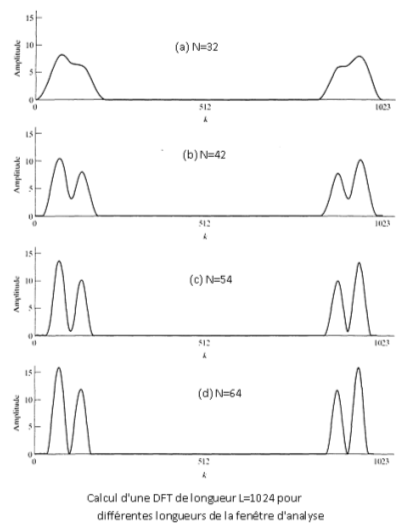
\includegraphics[scale=0.4]{ch5/image7}
	\captionof{figure}{\ }
	\end{center}
	
	
	
	
	
	
	
	
	
	
	
	
	
	
	
	
	
	
	
	
	
	
	
	
